% !TEX program = xelatex
% Figure 1 (CONSORT 형식, nested CV): 실험16 Late Fusion · Gated Late Fusion 의 환자 선정·분할 흐름도.
% 흰 상자 + 검은 실선 + 왼쪽 제외 상자, Times New Roman.
% 서체: Times New Roman 은 ~/.local/share/fonts 에 사용자 설치(MS 라이선스라 저장소에 넣지 않는다).
%       없는 장비에서는 같은 Times 계열 Nimbus Roman 으로 자동 대체된다.
% 수치 출처(2026-10-16 재계산):
%   321 / 64 / 9 / 8 / 2 -> 238   src/sclc/cohort.py::build_manifest()  (consort 판과 같음)
%   LS 72, ES 166                  merged_tabular_with_reports.csv 'stage' (1 = LS, 2 = ES)
%   분할                            data/splits/gmu_nested_v1/fold_manifest.json (outer = trimodal_common_5fold_seed42_v1)
%     outer train 190-191 (OS 159-160, PFS 169-170) / outer test 47-48 (OS 39-40, PFS 42-43)
%     inner fit 120-122 (OS 101-102, PFS 104-110) / stop 22 (OS 18, PFS 18-21) / V 47-48 (OS 39-40, PFS 41-44)
%     inner 층화 = os_event (5 outer 모두 primary rule), fit/stop 분할도 os_event 층화
\documentclass[tikz,border=8pt,10pt]{standalone}
\usepackage{fontspec}
\IfFontExistsTF{Times New Roman}{\setmainfont{Times New Roman}}{\setmainfont{Nimbus Roman}}
\usetikzlibrary{arrows.meta,positioning}
\begin{document}
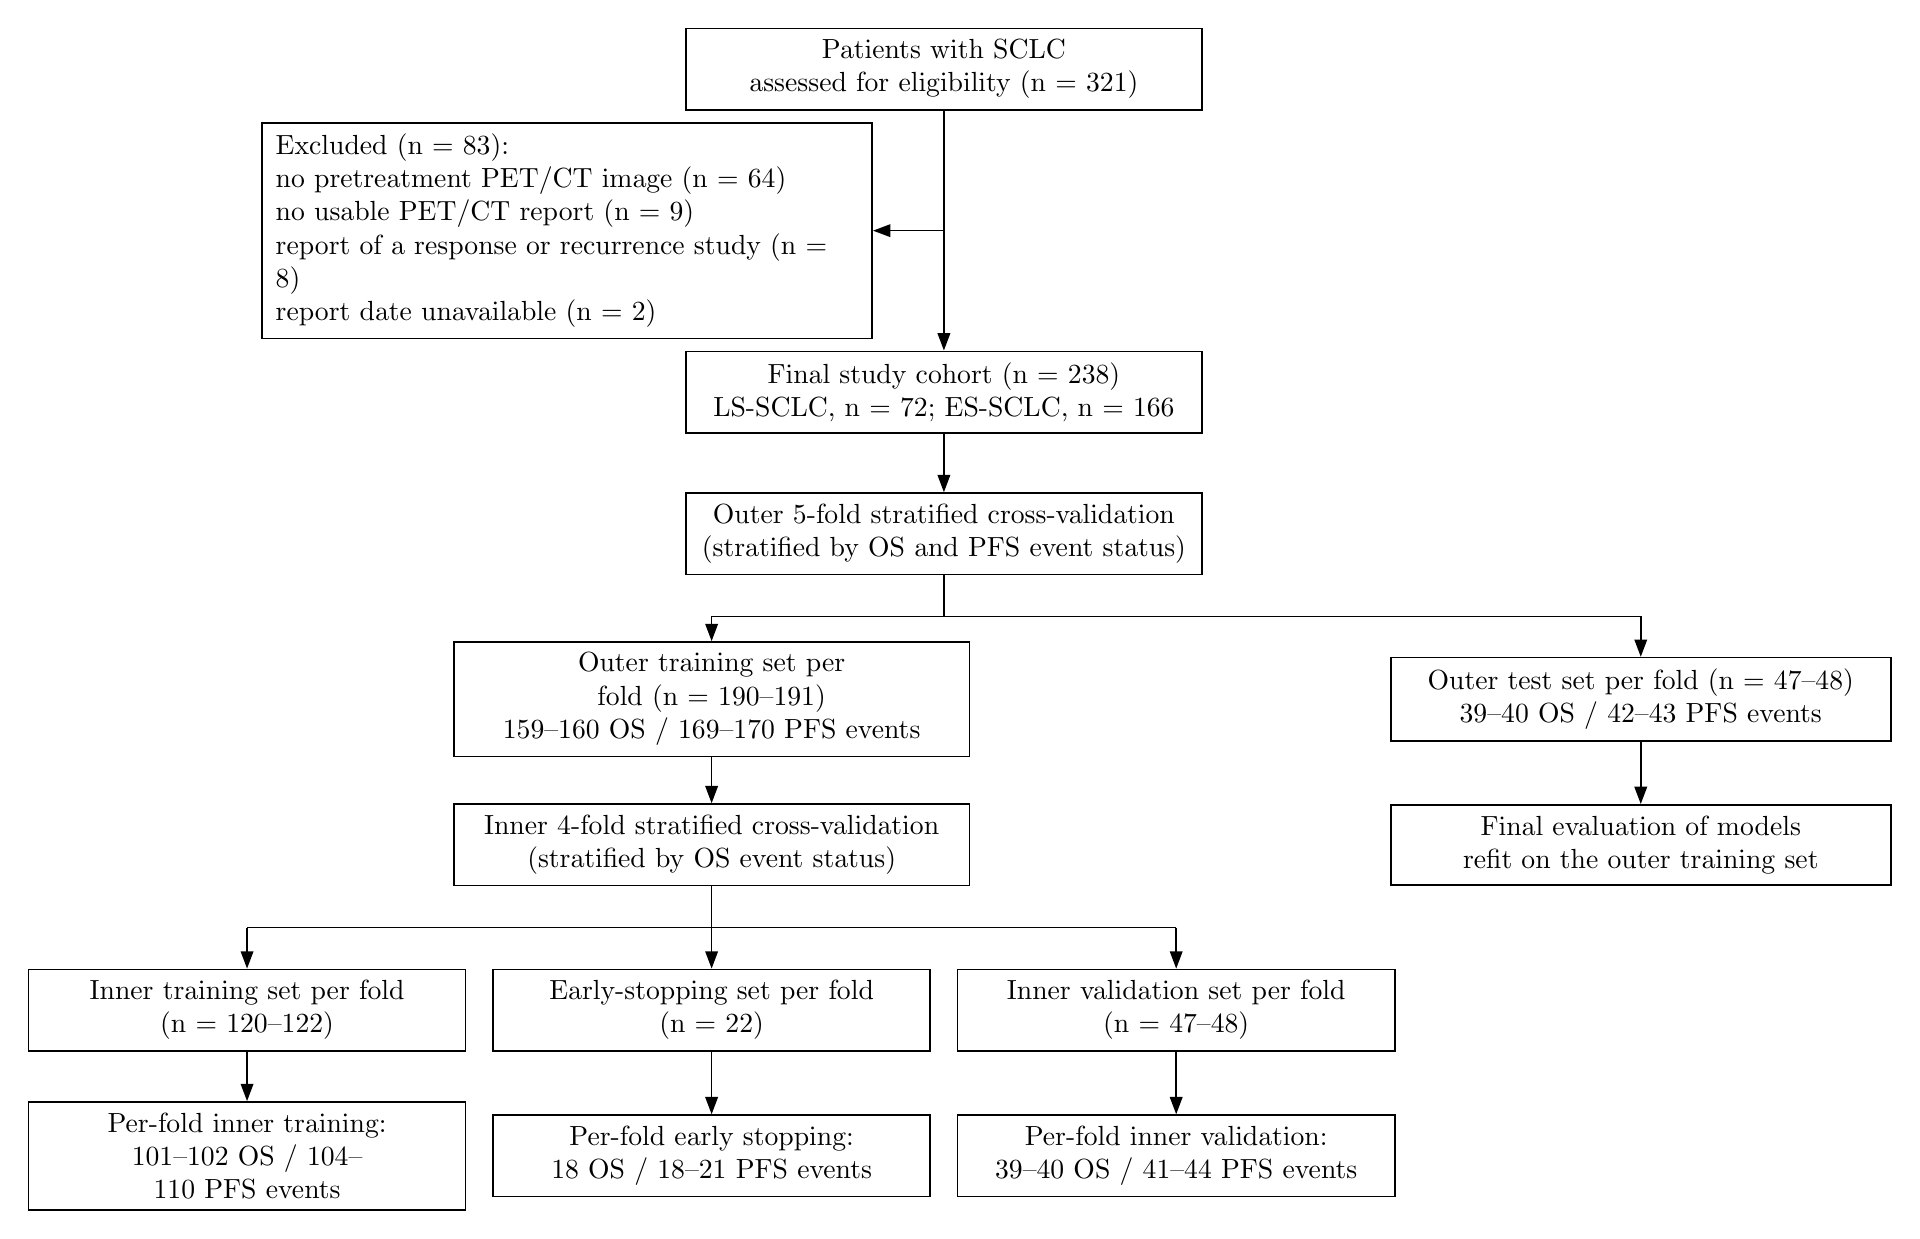
\begin{tikzpicture}[x=1cm,y=1cm,
  box/.style={draw=black, line width=0.6pt, fill=white, align=center,
              inner xsep=5pt, inner ysep=4pt, text width=#1},
  box/.default=62mm,
  excl/.style={box=74mm, align=left},
  sub/.style={box=52mm},
  arr/.style={draw=black, line width=0.6pt, -{Triangle[length=2.2mm,width=1.6mm]}},
  line/.style={draw=black, line width=0.6pt},
]

% ---------------- 선정 ----------------
\node[box] (all) at (0,0)
  {Patients with SCLC\\ assessed for eligibility (n = 321)};

\node[excl, anchor=east] (ex) at (-0.9,-2.05)
  {Excluded (n = 83):\\
   no pretreatment PET/CT image (n = 64)\\
   no usable PET/CT report (n = 9)\\
   report of a response or recurrence study (n = 8)\\
   report date unavailable (n = 2)};

\node[box] (final) at (0,-4.1)
  {Final study cohort (n = 238)\\ LS-SCLC, n = 72; ES-SCLC, n = 166};

% ---------------- outer 교차검증 ----------------
\node[box] (cv) at (0,-5.9)
  {Outer 5-fold stratified cross-validation\\ (stratified by OS and PFS event status)};

\node[box] (otr) at (-2.95,-8.0)
  {Outer training set per fold (n = 190--191)\\ 159--160 OS / 169--170 PFS events};
\node[box=60mm] (ote) at (8.85,-8.0)
  {Outer test set per fold (n = 47--48)\\ 39--40 OS / 42--43 PFS events};

% ---------------- inner 교차검증 (outer training set 안) ----------------
\node[box] (icv) at (-2.95,-9.85)
  {Inner 4-fold stratified cross-validation\\ (stratified by OS event status)};

\node[sub] (itr) at (-8.85,-11.95) {Inner training set per fold\\ (n = 120--122)};
\node[sub] (ist) at (-2.95,-11.95) {Early-stopping set per fold\\ (n = 22)};
\node[sub] (iva) at (2.95,-11.95)  {Inner validation set per fold\\ (n = 47--48)};

\node[sub] (itrd) at (-8.85,-13.8) {Per-fold inner training:\\ 101--102 OS / 104--110 PFS events};
\node[sub] (istd) at (-2.95,-13.8) {Per-fold early stopping:\\ 18 OS / 18--21 PFS events};
\node[sub] (ivad) at (2.95,-13.8)  {Per-fold inner validation:\\ 39--40 OS / 41--44 PFS events};

% outer test 열: 최종 평가
\node[box=60mm] (eval) at (8.85,-9.85)
  {Final evaluation of models\\ refit on the outer training set};

% ---------------- 화살표 ----------------
\draw[arr] (all) -- (final);
\draw[arr] (0,-2.05) -- (ex.east);
\draw[arr] (final) -- (cv);

\draw[line] (cv.south) -- (0,-6.95);
\draw[line] (-2.95,-6.95) -- (8.85,-6.95);
\draw[arr] (-2.95,-6.95) -- (otr.north);
\draw[arr] (8.85,-6.95) -- (ote.north);

\draw[arr] (otr) -- (icv);
\draw[arr] (ote) -- (eval);

\draw[line] (icv.south) -- (-2.95,-10.9);
\draw[line] (-8.85,-10.9) -- (2.95,-10.9);
\draw[arr] (-8.85,-10.9) -- (itr.north);
\draw[arr] (-2.95,-10.9) -- (ist.north);
\draw[arr] (2.95,-10.9) -- (iva.north);

\draw[arr] (itr) -- (itrd);
\draw[arr] (ist) -- (istd);
\draw[arr] (iva) -- (ivad);

\end{tikzpicture}
\end{document}
